\section{Fault check of digital circuit}

\renewcommand{\CURPATH}{MaxSMT/fault_check}

Donald Knuth's TAOCP section 7.2.2.2 has the following exercise.

\begin{figure}[H]
\centering
\frame{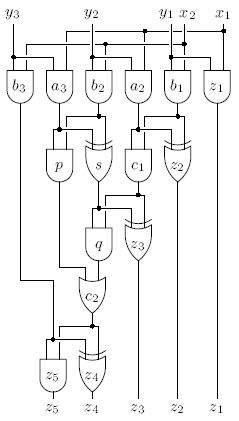
\includegraphics[scale=0.85]{\CURPATH/circuit.png}}
\end{figure}

Find a way to check, if it was soldered correclty, with no wires stuck at ground (always 0) or current (always 1).
You can just enumerate all possible inputs (5) and this will be a table of correct inputs/outputs, 32 pairs.
But you want to make fault check as fast as possible and minimize test set.

This is almost a problem I've been writing before: \ref{set_cover}.

We want such a test set, so that all gates' outputs will output 0 and 1, at least once.
And the test set should be as small, as possible.

The source code is very close to my previous example...

\lstinputlisting[style=custompy]{\CURPATH/1.py}

The output:

\lstinputlisting{\CURPATH/out.txt}

This is it, you can test this circuit using just 3 test vectors: 01111, 10001 and 11011.

However, Donald Knuth's test set is bigger: 5 test vectors, but his algorithm also checks "fanout" gates (one input, multiple outputs), which also may be faulty.
I've omitted this for simplification.

